% IEEE ESL letter draft (4 pages). Compile on Overleaf with IEEEtran.
% Numbers marked <...> are filled from device measurements (2026-11-05/06).
\documentclass[journal,letterpaper]{IEEEtran}

\usepackage{cite}
\usepackage{amsmath,amssymb}
\usepackage{graphicx}
\usepackage{booktabs}
\usepackage{array}
\usepackage{url}

\begin{document}

\title{Fully-Resident Weight Storage for Mixed-Precision\\ SLM Inference on a 32-MB PSRAM MCU}

\author{<Author Name>%
\thanks{<Affiliation, city, country; e-mail>. Manuscript received <date>.}}

\markboth{IEEE Embedded Systems Letters}%
{<Author>: Fully-Resident Weight Storage for Mixed-Precision SLM Inference}

\maketitle

\begin{abstract}
We show that mixed-precision quantization enables fully-resident weight storage of a dense
small language model (SLM) on a 32-MB PSRAM microcontroller. A 63.91M-parameter model
quantized to q3e4 (embedding/output q4, attention and FFN q3) occupies \textbf{27.3 MiB}
and runs entirely in on-package PSRAM with a \textbf{192-token} context window (FP16 K/V cache) and no host
at inference time. Measured decode throughput is \textbf{0.465 tok/s} (2.15 s/token) after
int16-activation, zero-copy packed GEMV plus activation-quantization hoisting, a
\textbf{2.61$\times$} cumulative speedup over the scalar baseline (2.13$\times$ from the
storage-format change and 1.23$\times$ from the hoisting pass); the GEMV kernel dominates
decode time, so kernel-level gains pass through almost unchanged to end-to-end latency. A pre-registered
accuracy lower bound (fixed-text cross-entropy within 1.15$\times$ of q4, plus a deterministic
30-prompt rule score $\geq 80\%$) separates the feasible configurations: q2 crosses the
accuracy cliff, q4 exceeds the 32-MB budget, and mixed/q3e4 both meet the bound while q3e4
keeps about four times more PSRAM headroom and is selected for deployment. All arithmetic is
auditable line by line and the artifact is open.
\end{abstract}

\begin{IEEEkeywords}
Edge AI, on-device inference, large language models, mixed-precision quantization, PSRAM,
microcontrollers, memory capacity.
\end{IEEEkeywords}

\section{Introduction}
\IEEEPARstart{P}{utting} an entire dense language model on a microcontroller is a capacity
problem before it is a compute problem. On a fixed 32-MB PSRAM budget, a 63.91M-parameter
SLM needs about 244~MiB in FP16 and 128~MiB in INT8, both far beyond on-package memory;
weights must therefore be compressed until they fit, and any configuration that does not fit
is simply not a candidate, regardless of its arithmetic quality.

Prior work avoids this wall~\cite{memorywall} in two ways. A 180.9M-parameter MoE design (p-for-llm)~\cite{pforllm} trades
dense residency for sparsity: only the routed experts are active, its $\sim$44~MiB of state
is split between flash XIP and PSRAM, and part of the PSRAM weights are transferred from a
host over USB at boot, so the host is absent during inference yet still required at startup;
its $\sim$9~tok/s reflects top-1 routing over 29 experts per layer. The PIE series~\cite{pie} instead
accelerates kernels on models far below the capacity boundary (0.61$\rightarrow$4.31~tok/s)
and does not address how much dense model can reside. A recent survey of MCU LLM systems~\cite{survey}
finds fully-on-chip evidence only at the 256--412~KB scale and one 5.81~MB ternary ViT with
external PSRAM; a fully-resident \emph{dense} 27.3~MiB model on an ESP32-class device falls
in a region that is not covered. For scale, an ESP32-S3 board has been reported at 22.6~tok/s on a TinyStories-scale model~\cite{edgebench}.

This letter answers two questions within one concrete design point: how far a dense SLM can be
compressed and still reside fully in 32~MB of PSRAM, and what latency that residency costs once
the storage problem is solved. We quantify the deployment frontier with a pre-registered
accuracy bound, measure the decode-time split between GEMV and the rest of the forward pass,
and show that the GEMV kernel---not PSRAM bandwidth---dominates latency, which is why a 2.13$\times$
kernel optimization appears almost one-to-one at the system level. We do not claim a new
quantization method or a new system architecture: the contribution is an auditable capacity point,
a measured latency-cost attribution, and a reproducible artifact.

\section{Method}
\textbf{Quantization scheme.} Following the group-wise post-training quantization line~\cite{gptq,awq,llmint8}, q3e4 stores the token embedding and the tied output layer at
q4\_0 (18 bytes per 32 weights: one fp16 block scale plus 16 packed nibbles) and all attention
and FFN linear projections at q3\_0 (14 bytes per 32 weights: fp16 scale plus 12 packed
3-bit values). Activations are quantized to int16 per GEMV call~\cite{int16}; RMSNorm weights, biases and
the KV cache remain FP32. A KMCU image is a single flat file with a 4,480-byte header followed
by per-tensor packed blocks; the q3e4 image is 28,632,448 bytes (27.3~MiB).

\textbf{Accuracy lower bound (pre-registered).} A configuration is deployable only if it
simultaneously satisfies (i) per-token cross-entropy on a fixed text within 1.15$\times$ of the
q4 reference, and (ii) a deterministic rule score of at least 80\% on 30 fixed prompts. The
thresholds were fixed before measuring q3e4 and are not adjusted afterwards. The q4 reference
cannot run on the device (36.0~MB exceeds the budget), so it is simulated on a host with the
identical block-32 recipe; the same host simulation reproduces q3e4, and host/device
cross-checking bounds the simulation error (Sec.~III).

\textbf{Bit allocation rationale.} The embedding and output matrix (6400$\times$768) is kept at
q4 because it carries lexical identity and is reused by the tied head, while the FFN projections
are the largest parameter group and therefore the main compression lever; attention projections
are compressed less aggressively than FFN only to the extent the budget allows. The resulting
q3e4 point is a capacity calculation, not a claim that embeddings are universally more
sensitive.

\textbf{Zero-copy packed GEMV.} Dequantizing to an expanded FP32/INT8 copy would double the
resident footprint and add per-element traffic. Instead, the packed image is used in place:
each 32-weight block is read from PSRAM, unpacked on the fly into signed integers, and dotted
with the int16 activation vector; the fp16 block scale is applied to the integer partial sum.
The inner loops read 32-bit words rather than individual 3-bit fields. The same kernel serves
all linear layers and the tied output head, so the storage format and the compute path are
consistent by construction.

\textbf{Context and KV budget.} The deployed context is 192 tokens with FP16 K/V caches:
$2 \times 8 \times 192 \times 4 \times 96 \times 2$~B $=$ 2,359,296~B, i.e. the same PSRAM as a
96-token FP32 cache (for reference, 96 tokens with FP32 K/V was the earlier configuration;
Sec.~III reports the measured effect of the FP16 cache).

\textbf{Model.} The weights are trained from scratch on a local 12-GB GPU: pre-training
(39,695 steps, final loss 2.01) and supervised fine-tuning (56,608 steps, final loss 1.71),
followed by a separate LoRA reproduction experiment (rank 16, 7,900 steps, loss 1.2564) and
the q3e4 quantization described above. The architecture follows Qwen3-style QK-norm~\cite{qwen3} and the MiniMind training recipe~\cite{minimind}; a QK-norm correction in the deployed kernel is an
enabling fix, not a contribution.
\textbf{Hardware and integration.} The host is an ALINTEK ESP32-P4 board (360~MHz, 16~MB flash,
32~MB PSRAM)~\cite{psram}; the 28.63~MB KMCU image and tokenizer live on a microSD card and are
streamed into PSRAM at boot. The board acts as a USB host for the HachimoDock desktop
pet~\cite{hachimodock} through a CH343 bridge at 4~Mbaud: pet input events arrive as JSON
messages and generated replies are returned as incremental \texttt{speech/text} bubbles. All
inference runs on the board; no PC or network participates after flashing.

\section{Results}
\textbf{Memory budget (Table~\ref{tab:budget}).} All weights and caches are allocated once at
boot and their sizes are auditable: the q3e4 image (28,632,448~B) plus the KV cache
(2,359,296~B) plus small internal-RAM workspaces leave 2,352,828~B of PSRAM free after KV
initialization, measured at runtime.

\begin{table}[t]
\centering
\caption{Deployed memory budget on a 32-MB PSRAM ESP32-P4 (measured).}
\label{tab:budget}
\footnotesize
\setlength{\tabcolsep}{2.5pt}
\begin{tabular}{@{}lr@{}}
\toprule
Item & Bytes \\
\midrule
q3e4 weights & 28,632,448 (27.3 MiB) \\
KV (192 tok, FP16) & 2,359,296 \\
Norm arena (int.\ RAM) & 58,368 \\
Scratch+act (int.\ RAM) & 52,608 \\
PSRAM free after KV & 2,352,828 \\
\midrule
PSRAM total & $\leq$ 33,554,432 \\
\bottomrule
\end{tabular}
\end{table}

\begin{figure*}[t]
\centering
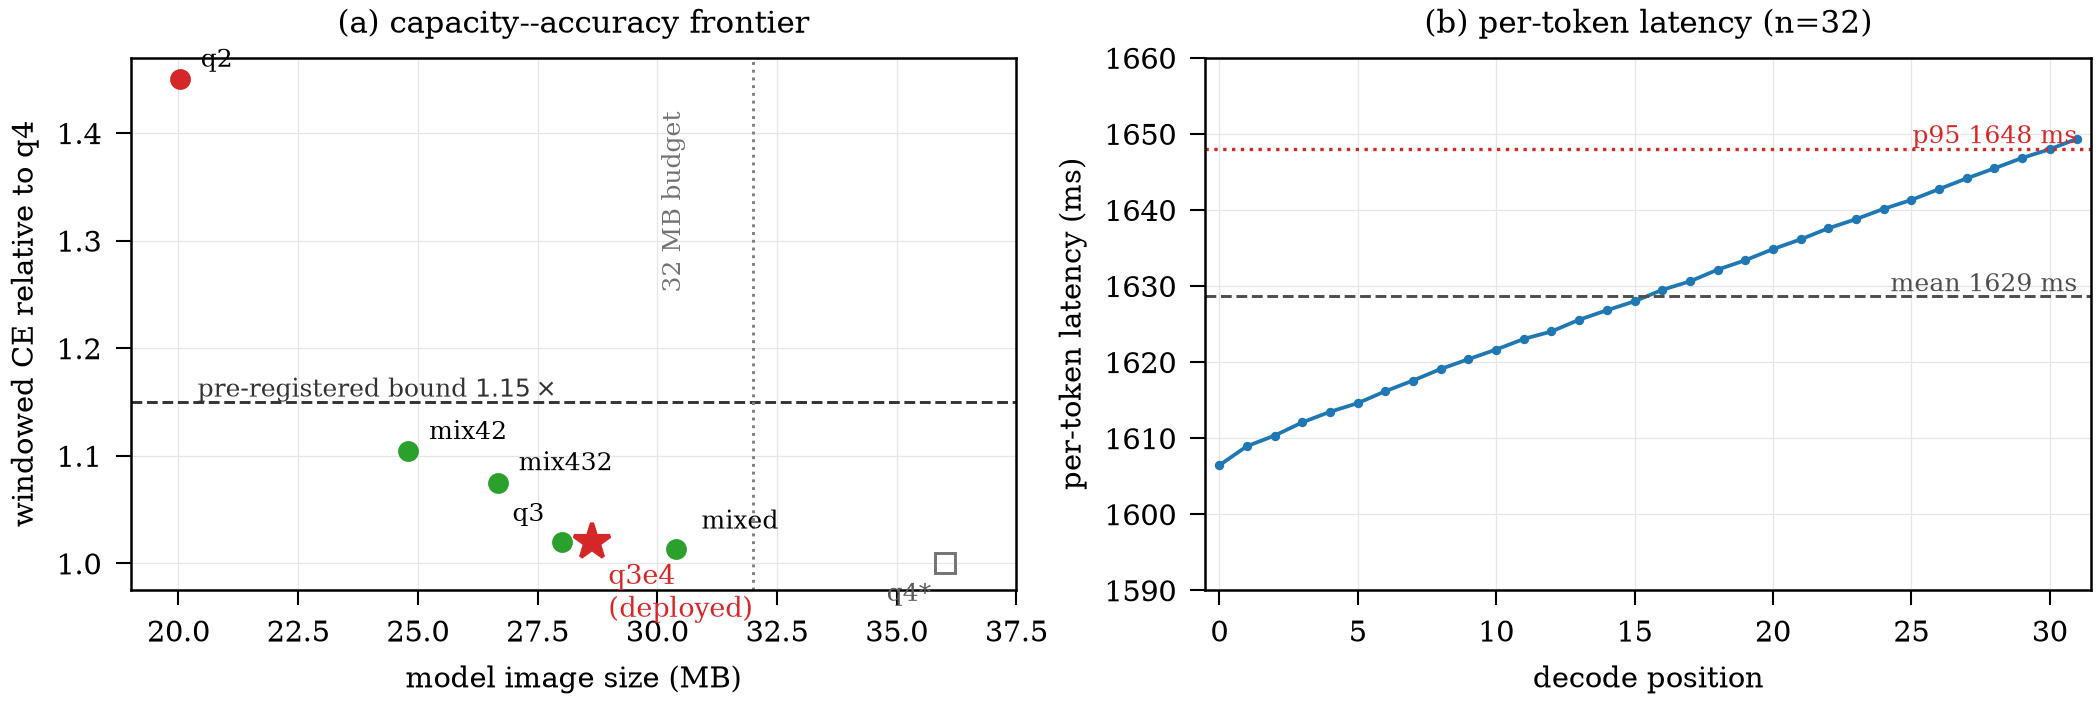
\includegraphics[width=\textwidth]{figures/fig_frontier_latency.png}
\caption{(a) Capacity--accuracy frontier under the 32-MB PSRAM budget: windowed CE
relative to q4 versus model image size, with the pre-registered $1.15\times$ bound and the
memory cliff; q3e4 is the deployment point. (b) Per-token decode latency over one 32-token
run (mean 2,170~ms, p95 2,189~ms); the mild upward slope is attention over the growing K/V
cache.}
\label{fig:frontier}
\end{figure*}

\textbf{Decode latency and GEMV share (Table~\ref{tab:gemv}, Fig.~\ref{fig:frontier}b).} The storage-format change
(int16 activations + zero-copy packed weights) reduces decode from the 5,622~ms/token
scalar-expanded baseline to 2,639~ms/token (0.379~tok/s), a 2.13$\times$ kernel-level gain.
Hoisting the per-token activation quantization out of the 6,400-row output-head loop and
replacing per-weight offsets by block-sum corrections lowers it to
\textbf{2,152~ms/token (0.465~tok/s)}, i.e. 2.61$\times$ cumulative, with bit-identical CE.
Instrumenting the packed GEMV path with cycle counters gives a GEMV share $r=0.988$ on the
2,639-ms build; after hoisting, the measured share is $r=0.985$. For the format change, Amdahl's law with $r=0.988$ and a 2.13$\times$ kernel gain predicts $1/((1-r)+r/2.13)=1.97\times$ end-to-end (observed 2.13$\times$); for the hoisting pass, $r=0.985$ and a 1.23$\times$ kernel gain predict 1.22$\times$ (observed 1.23$\times$), so kernel gains pass through almost unchanged. Counting one full read
of packed weights (28.63~MB) plus one complete KV pass (2.36~MB) gives 30.99~MB/token, i.e.
13.3--14.4~MB/s at the two operating points, while the weight-only rate during GEMV is
10.98--13.3~MB/s---far below the 95.9~MB/s sequential-read microbenchmark. The scalar
unpack-plus-dot instruction stream, not memory bandwidth, is therefore the limiting factor:
a bandwidth-bound design would call for a different storage format, whereas an
instruction-bound one motivates kernel vectorization or wider unpacking.

\begin{table}[t]
\centering
\caption{Decode-time ablation (measured on device).}
\label{tab:gemv}
\footnotesize
\setlength{\tabcolsep}{2.5pt}
\begin{tabular}{@{}lrrrr@{}}
\toprule
Config & ms/tok & Speedup & $r$ & MB/s \\
\midrule
Scalar float, expanded & 5,622 & 1$\times$ & -- & -- \\
int16 + packed & 2,639 & 2.13$\times$ & 0.988 & 10.98 \\
+ hoisted quant. & \textbf{2,152} & \textbf{2.61$\times$} & 0.985 & 13.5 \\
\bottomrule
\end{tabular}
\end{table}

\textbf{FP16 K/V cache.} Replacing the FP32 K/V cache with FP16 storage doubles the context to
192 tokens at the same 2,359,296~B. Window-0 CE changes from 6.662094 to 6.660667
($\Delta=0.0014$, 0.02\%) and decode time from 2,152 to 2,154~ms/token (within run-to-run
noise), so the larger context is adopted at no measurable cost. The doubled context also pays
off in modeling: on the same token prefix, one 192-token window scores CE 5.970 versus 7.014
for resetting every 96 tokens (190/191 targets), i.e. about a 15\% reduction in CE
(PPL 392 vs.\ 1,107).

\textbf{Accuracy frontier (Table~\ref{tab:frontier}, Fig.~\ref{fig:frontier}a).} Host simulation with the identical windowed recipe (each 96-token window
scored independently, matching the deployed context) places q4 at CE $=6.949$ (PPL 1,042) and
q3e4 at 7.087 (1.020$\times$, PPL 1,197); q2 reaches 10.074 (1.450$\times$, PPL 23,710), clearly
beyond the pre-registered bound. On a second, English public corpus (Apache-2.0 license text,
288 tokens) the ordering is unchanged: q3e4 5.676 (1.048$\times$ of q4) versus q2 9.905
(1.829$\times$). The device reproduces q3e4 window-by-window with a host/device CE difference
below 0.001, which validates the host-simulated q4 reference, and the 30-prompt rule score is
80\% for q3e4 versus 0\% for q2 (the fp32 reference also scores 80\%). On the same capacity budget, mixed
(embedding/attention q4, FFN q3; 30.40~MB) also satisfies the accuracy bound (CE 7.037,
1.013$\times$), but it leaves only about 0.58~MB of PSRAM after the KV cache, whereas q3e4 leaves
2.35~MB. We therefore report a \emph{feasibility frontier} rather than a unique configuration:
both mixed and q3e4 satisfy the pre-registered bound (mixed is even slightly more accurate and
faster on this kernel), and q3e4 is selected as the deployment point for its four-fold larger
runtime headroom under heap fragmentation and USB/protocol activity.

\begin{table}[t]
\centering
\caption{Capacity--accuracy frontier (32-MB PSRAM; host simulation, windowed CE, same recipe).}
\label{tab:frontier}
\footnotesize
\setlength{\tabcolsep}{2.5pt}
\begin{tabular}{@{}lrrrrr@{}}
\toprule
Config & Size (B) & CE & CE/q4 & Rule & ms \\
\midrule
q2 & 20,030,848 & 10.074 & 1.450 & 0\% & 1,352 \\
q3 & 28,018,048 & 7.090 & 1.020 & -- & -- \\
\textbf{q3e4} & \textbf{28,632,448} & \textbf{7.087} & \textbf{1.020} & \textbf{80\%} & \textbf{2,152} \\
mixed & 30,401,920 & 7.037 & 1.013 & 73.3\% & 2,017 \\
q4 & 36,005,248 & 6.949 & 1.000 & 73.3\% & n/a \\
\bottomrule
\end{tabular}
\end{table}

Two further configurations with larger headroom also satisfy the bound but trade accuracy:
mix42 (24.80~MB; embedding/attention q4, all FFN q2) reaches CE 7.673 (1.104$\times$ of q4) and a
60.0\% rule score, and mix432 (26.67~MB; FFN down q3) reaches 7.467 (1.075$\times$) and 66.7\%,
so the frontier below q3e4 is graded rather than a single jump.

\textbf{Positioning (Table~\ref{tab:compare}).} The closest points are a sparsity-assisted MoE
with partial residency and a boot-time host transfer, and vector-kernel acceleration on models
well below the capacity boundary. We do not compare throughput directly: the table positions
constraint differences, and the reported throughputs are cited as reported by their authors.

\begin{table}[t]
\centering
\caption{Constraint comparison (throughput values as reported, not reproduced).}
\label{tab:compare}
\footnotesize
\setlength{\tabcolsep}{2.5pt}
\begin{tabular}{@{}lrrr@{}}
\toprule
Work & Model & Residency / boot & tok/s \\
\midrule
p-for-llm & 180.9M MoE & partial; USB boot & $\sim$9 \\
PIE & -- & kernel accel.; no capacity & 0.61--4.31 \\
\textbf{This work} & 63.91M dense & \textbf{full 27.3 MiB; no host} & \textbf{0.465} \\
\bottomrule
\end{tabular}
\end{table}

\textbf{End-to-end and startup.} Weight loading from a TF card takes about 20.6~s, dominated by
the card read; the packed image needs no post-load unpacking. Over 40 measured decode steps,
per-token latency is 2,166.6~ms on average (median 2,164.4~ms, p95 2,189.0~ms, std.\ 13.1~ms),
i.e. a narrow distribution without long tails; latency grows by about 2\% from position 0 to 31
as attention reads a longer K/V cache. Prompt prefill is processed token-by-token with the same
kernel (no batched prefill), so a short event-driven query plus a 32-token reply takes on the
order of one to two minutes; this is consistent with the intended single-turn,
non-conversational usage and is reported as a limitation rather than a capability. The mixed
configuration (30.40~MB) also boots and generates in the full standalone firmware (model load,
pet-host protocol stack, and local generation), confirming that the frontier points other than
q3e4 are deployable rather than merely measurable.

\section{Discussion and Limitations}
The measured split changes the design story: the deployment is GEMV-bound ($r=0.988$ before hoisting; 0.985 after), and the
scalar unpack/dot instruction stream is the throughput limiter, not the PSRAM bandwidth. The
practical consequence is that the 2.13$\times$ kernel gain survives at the system level, and
further gains should come from wider unpacking or ISA-level vectorization rather than from
reducing bytes read. The 192-token context is obtained at no extra memory by storing the K/V cache in FP16
(2.25~MiB for 192 tokens); measured windowed CE changes by 0.0014 and decode time is
statistically unchanged, so the FP16 cache is adopted for deployment while FP32 K/V at 96
tokens remains a conservative fallback. The model itself is deliberately small and trained on a single local GPU; its absolute
quality is not the claim---accuracy measurements only delimit the feasible set. We report no
energy-per-token figure (no power meter was available) and no standard benchmark score; a fixed
held-out text and a deterministic rule set keep the comparison auditable but bound external
validity. The usage model is single-turn: prompt prefill is token-by-token and replies are
short, so the reported throughput is not a conversational latency. The artifact,
training logs, evaluation scripts and the self-trained q3e4 image are public for reproduction.

\textbf{Reproducibility and artifact.} The public repository contains the self-trained q3e4 image
(SHA-256 \texttt{feb574f9\ldots}), the firmware sources for the packed GEMV kernel and the USB
host bridge, the 30 evaluation prompts with their rule checker, the windowed-CE scripts, the
held-out text and token ids, and the five alternative quantized images used for the frontier
(mixed, q3, q4, mix42, mix432). Every number in Tables~I--IV can be regenerated from these
files; the host simulation uses the identical block-32 recipe as the C kernel, and the
host/device agreement above bounds the simulation error. The peak-PSRAM and bandwidth
microbenchmarks are part of the measurement firmware and are documented in the runbook.

\section{Conclusion}
A 63.91M dense SLM can reside fully in 32~MB of PSRAM at 27.3~MiB with a 192-token context and
no host participation, and the resulting latency is dominated by the packed GEMV kernel rather
than by memory bandwidth, so kernel-level work transfers almost directly to end-to-end speed.
The capacity--accuracy frontier, with q2 beyond the accuracy cliff and q4 beyond the budget, is
measured under a pre-registered bound and is reproducible from the public artifact.

\section*{Acknowledgment}
The author used the DeepSeek Harness AI coding agent (DeepSeek model) to assist with the
ESP32-P4 firmware implementation (model loading, packed-weight GEMV kernels, USB host protocol
bridge), quantization and measurement tooling (Sections II--III), experiment automation, and
manuscript editing. The AI system is not an author. The author independently verified all
generated code, measurements and text and takes full responsibility for the accuracy,
originality and integrity of this work.

\begin{thebibliography}{18}
\bibitem{pforllm} cyfrit, ``PFor: Offline 180.9M-parameter LLM and agent inference on ESP32-P4,'' GitHub repository, 2026. [Online]. Available: https://github.com/cyfrit/p-for-llm
\bibitem{pie} ``From 0.61 to 4.31 tok/s: A complete record of MCU-side LLM inference level-four optimization,'' EEWorld forum, Oct. 2026. [Online]. Available: \url{https://en.eeworld.com.cn/bbs/forum.php?mod=viewthread&tid=1369555}
\bibitem{survey} M.~R.~Ramdhani, ``Language and transformer models with ESP32-class microcontrollers: A systematic review of hybrid deployment and on-device optimization,'' 2026. [Online]. Available: https://journals.unpad.ac.id/ijmt/article/view/72405
\bibitem{qwen3} Qwen Team, ``Qwen3 technical report,'' arXiv:2505.09388, 2025.
\bibitem{gptq} G.~Frantar, S.~Ashkboos, T.~Hoefler, and D.~Alistarh, ``GPTQ: Accurate post-training quantization for generative pre-trained transformers,'' in \emph{Proc. ICLR}, 2023.
\bibitem{awq} J.~Lin \emph{et al.}, ``AWQ: Activation-aware weight quantization for on-device LLM compression and acceleration,'' in \emph{Proc. MLSys}, 2024.
\bibitem{llmint8} T.~Dettmers, M.~Lewis, Y.~Belkada, and L.~Zettlemoyer, ``LLM.int8(): 8-bit matrix multiplication for transformers at scale,'' in \emph{Proc. NeurIPS}, 2022.
\bibitem{psram} Espressif Systems, ``ESP32-P4 technical reference manual,'' 2025.
\bibitem{minimind} Jingyaogong, ``MiniMind: train a small language model from scratch,'' GitHub repository, 2025. [Online]. Available: https://github.com/jingyaogong/minimind
\bibitem{memorywall} W.~Wulf and S.~McKee, ``Hitting the memory wall: Implications of the obvious,'' \emph{ACM SIGARCH Comput. Archit. News}, vol.~23, no.~1, pp.~20--24, 1995.
\bibitem{edgebench} ``LLM on a microcontroller: ESP32-S3 at 22.6 tok/s,'' technical report, 2026. [Online]. Available: https://insiderllm.com/pdfs/llm-on-microcontroller-esp32-s3.pdf
\bibitem{int16} B.~Jacob \emph{et al.}, ``Quantization and training of neural networks for efficient integer-arithmetic-only inference,'' in \emph{Proc. CVPR}, 2018.
\bibitem{ternaryvit} S.~Ma, H.~Wang, L.~Ma, L.~Wang, W.~Wang, S.~Huang, L.~Dong, R.~Wang, J.~Xue, and F.~Wei, ``The era of 1-bit LLMs: All large language models are in 1.58 bits,'' arXiv:2402.17764, 2024.
\bibitem{hachimodock} Y.~Wang \emph{et al.}, ``HachimoDock: An open-source desktop AI hardware,'' GitHub repository, 2026. [Online]. Available: https://github.com/YizhengWw/HachimoDock
\end{thebibliography}

\end{document}
